\chapter{神经网络入门}

文章参考:\url{http://blog.csdn.net/zzwu/article/details/574931}

\section{生物学的大脑}
大脑是一块灰色的、像奶冻一样的东西。它并不像脑中的CPU那样,利用单个或少数几个处理单元来进行工作。如果你有一具新鲜地保存到福尔马林中的尸体,用一把锯子小心地将它的头骨锯开,搬掉头盖骨后,你就能看到熟悉的脑组织皱纹。大脑的外层象一个大核桃那样,全部都是起皱的[图0左],这一层组织就称皮层(Cortex)。如果你再小心地用手指把整个大脑从头颅中端出来,再去拿一把外科医生用的手术刀,将大脑切成片,那么你将看到大脑有两层: 灰色的外层(这就是“灰质”一词的来源,但没有经过福尔马林固定的新鲜大脑实际是粉红色的。如图~\ref{大脑皮层解剖图}) 和白色的内层。灰色层只有几毫米厚,其中紧密地压缩着几十亿个被称作neuron(神经细胞、神经元)的微小细胞。白色层在皮层灰质的下面,占据了皮层的大部分空间,是由神经细胞相互之间的无数连接线组成(但没有神经细胞本身,正如印刷电路板的背面,只有元件的连线,而没有元件本身那样,译注)。皮层象核桃一样起皱,这可以把一个很大的表面区域塞进到一个较小的空间里。这与光滑的皮层相比能容纳更多的神经细胞。人的大脑大约含有10G(即100亿)个这样的微小处理单元;一只蚂蚁的大脑大约也有250,000个。
\begin{figure}[H]
  \centering
  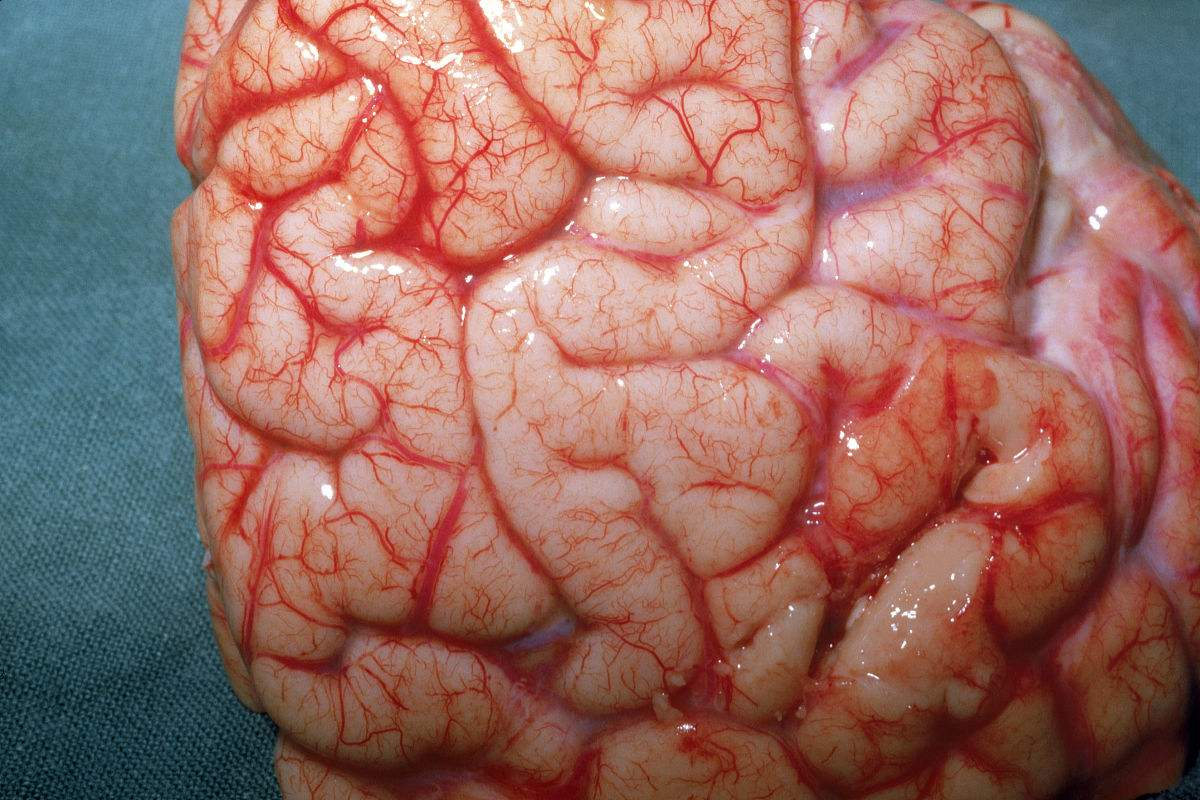
\includegraphics[width=10cm]{Figures/大脑皮层解剖图.jpg}
  \caption{大脑皮层解剖图}\label{大脑皮层解剖图}
\end{figure}

